\documentclass[12pt]{article}

% --- Preamble ---
\usepackage[utf8]{inputenc}
\usepackage[T1]{fontenc}
\usepackage{lmodern}
\usepackage{amsmath, amssymb}
\usepackage{graphicx}
\usepackage{geometry}
\geometry{a4paper, margin=1in}
\usepackage{hyperref} % For clickable links
\usepackage{caption} % For figure and table captions
\usepackage{subcaption} % For subfigures
\usepackage{float}

% --- Document Information ---
\title{Student Attitudes and Usage Patterns of AI Tools in Higher Education}
\author{Mauricio Mossi \\ University of Florida \\ m.mossi@ufl.edu}
\date{\today}

% --- Abstract Environment ---
\usepackage{abstract}
\renewcommand{\abstractname}{Abstract}

% --- Sections and Subsections ---
\setcounter{secnumdepth}{2} % Number up to subsections
\setcounter{tocdepth}{2}    % Include up to subsections in the table of contents

% --- Begin Document ---
\begin{document}

% --- Title Page ---
\maketitle
\begin{abstract}
This study explores college students’ attitudes toward and usage of artificial intelligence (AI) tools in academic settings. Survey results from a diverse group of students reveal generally positive perceptions of AI, with most participants agreeing that these tools enhance learning and are readily accessible. Writing and editing emerged as the most common use, followed by research, studying, and problem solving. Differences in usage patterns were observed across academic disciplines, with engineering students showing a stronger belief in the relevance of AI to their field. These findings suggest that while AI is broadly embraced, its perceived value and applications vary by area of study, highlighting opportunities for more tailored AI integration in higher education.
\end{abstract}

% --- Table of Contents ---
\tableofcontents
\newpage

% --- Introduction ---
\section{Introduction}
\label{sec:introduction}
The integration of artificial intelligence (AI) into higher education has accelerated dramatically in recent years, transforming how students access information, complete assignments, and engage with academic content \cite{am}. AI tools such as ChatGPT, Grammarly AI, and others are now readily available to college students, offering functionalities that range from language generation to code assistance and data analysis. As these technologies become more embedded in academic routines, educators and institutions face urgent questions regarding how students are using these tools—and whether usage patterns vary by academic discipline \cite{pedro}.
Existing literature has examined general trends in student adoption of AI technologies. Studies have found that students often use AI tools to enhance productivity, brainstorm ideas, and assist with writing tasks \cite{lin}. However, much of the current research focuses on AI adoption in specific domains such as computer science or education, with limited attention paid to how students in different academic fields may engage with AI in unique ways. This disciplinary gap is important, as the perceived utility, appropriateness, and frequency of AI use likely differ between, for example, engineering students writing code and liberal arts students composing essays \cite{pedro}.
To address this gap, the present study explores AI usage patterns among college students across a range of academic disciplines. Specifically, it investigates which tools students use, how frequently they use them, the academic tasks for which they are used, and students’ perceptions of AI’s value and accessibility. By identifying potential disciplinary differences in AI engagement, this research contributes to a deeper understanding of how AI is shaping academic life and highlights implications for educators, policy makers, and future research.
The guiding research question is: What are the prevailing patterns of AI usage and attitudes among college students, and how do these differ across academic disciplines?

% --- Methods ---
\section{Methods}
\label{sec:methods}

\subsection{Participants}
\label{subsec:participants}
This study analyzed responses from a total of 43 college students, the majority of whom were enrolled at the University of Florida. While demographic details such as age and gender were not collected, participants were asked to self-identify their academic major by selecting one of six broad categories: Engineering, Business, Liberal Arts and Sciences, Health Professions, Law Professions, and Agriculture. These categories were chosen to capture a diverse range of academic disciplines. However, this categorization may have obscured differences between individual majors within a given category, presenting a limitation in the analysis of discipline-specific trends.

\subsection{Instruments}
\label{subsec:instruments}
To explore patterns of AI usage and attitudes among college students, and how these vary across academic disciplines, a five-question survey was developed to collect both quantitative and qualitative data. The first question asked participants to indicate their academic discipline using the predefined categories. The second assessed the frequency of AI use for academic purposes, using a five-point Likert scale ranging from “never” to “daily.”
The third question asked students to select from a list of AI tools and services they had used for academic purposes, including options such as ChatGPT, Grammarly, Claude, and others. The fourth question addressed the specific academic tasks for which students used AI, such as writing assignments, coding, research, or exam preparation.
The final question consisted of three attitudinal statements rated on a five-point Likert scale, ranging from “strongly disagree” to “strongly agree”. These statements gauged students’ perceptions of AI’s educational value, accessibility, and its relevance to their particular field of study.
Together, these items were designed to capture both the behaviors and perceptions of students engaging with AI tools in their academic work. A copy of the full survey is included in Appendix A

\subsection{Procedure}
\label{subsec:procedure}
The survey was administered through Qualtrics and distributed electronically over a one-week period. Recruitment was conducted via university-affiliated group chats and social media platforms to reach a wide range of students across disciplines.
Early in the distribution process, it became evident that responses were heavily skewed toward Engineering majors. To address this imbalance, targeted efforts were made to gather more responses from underrepresented fields. Despite these efforts, Engineering remained overrepresented, accounting for 46\% of the sample. This disproportion is acknowledged as a limitation when interpreting the findings.
Following data collection, responses were cleaned and analyzed using Qualtrics and Python’s Pandas library. The full code, dataset, and analysis can be accessed on GitHub (see Appendix B).




% --- Results ---
\section{Results}
Of the 43 total respondents, Engineering students made up the largest group with 18 participants, followed by 11 from Liberal Arts and Sciences, 5 each from Business and Health Professions, and 4 whose majors did not align with the listed categories (Figure 1).


\begin{figure}[htbp]
  \centering
  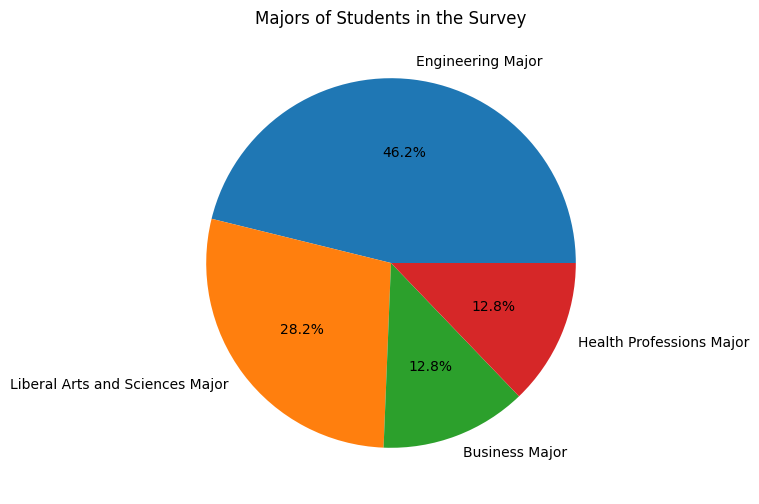
\includegraphics[width=0.6\textwidth]{fig1.png} % Replace with your figure file name
  \caption{Pie chart showing the distribution of participants by major.}
  \label{fig:example1}
\end{figure}

All participants reported using AI tools for academic purposes at least a few times per month. The most common frequency was “a few times per week,” selected by 15 participants. Nine reported using AI “nearly every day,” seven used it “daily,” and another seven indicated use “at least once a week.” No respondents selected “never” or “a few times a month,” indicating consistent and regular engagement with AI tools across the sample (Figure 2).

\begin{figure}[htbp]
  \centering
  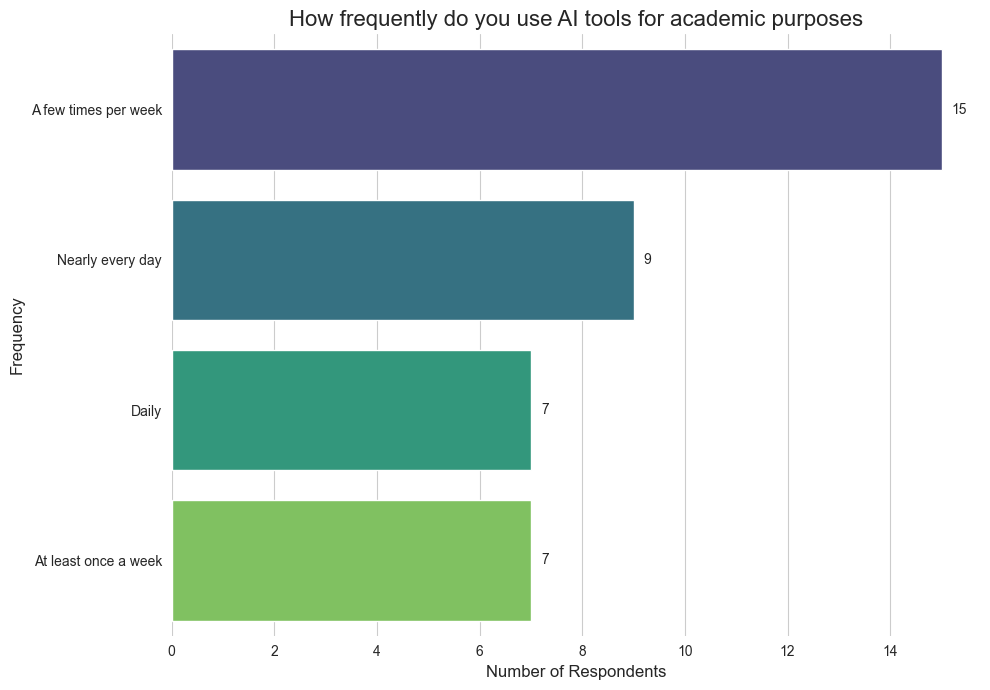
\includegraphics[width=0.7\textwidth]{fig2.png} % Replace with your figure file name
  \caption{Frequency chart of AI usage for academic purposes among participants.}
  \label{fig:example1}
\end{figure}

ChatGPT was by far the most widely used tool, reported by 38 out of 39 respondents (97\%). Gemini followed at 46\%, with other tools including Grammarly AI (26\%), Claude (23\%), DALL·E (15\%), and DeepSeek (13\%). Grok and GitHub Copilot were the least used, each mentioned by only one respondent (3\%) (Figure 3).

\begin{figure}[htbp]
  \centering
  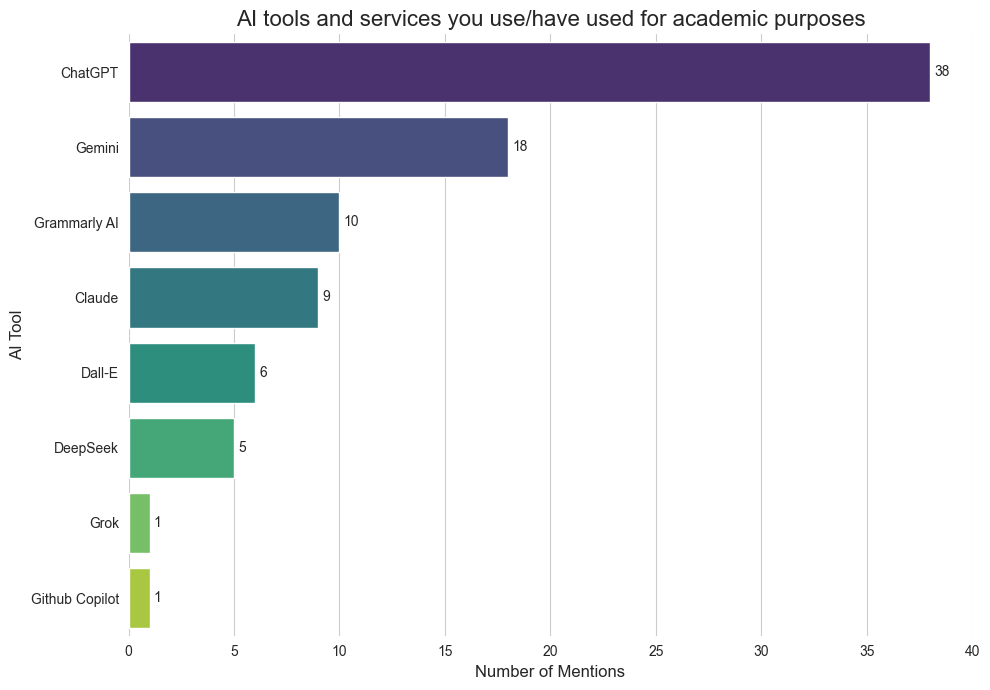
\includegraphics[width=0.7\textwidth]{fig3.png} % Replace with your figure file name
  \caption{Frequency chart of AI tool usage among participants.}
  \label{fig:example1}
\end{figure}

Breakdowns of AI tool usage by major (Figure 4) suggested differences in tool preference across disciplines. Among Engineering majors, 94\% reported using ChatGPT, with 39\% using Gemini and 28\% using Claude. In Liberal Arts and Sciences, all 11 participants reported using ChatGPT, 46\% used Gemini, and 27\% used Grammarly. While these patterns suggest some variation, limited sample sizes in several categories constrain broader generalizations.

% Example of two subfigures side-by-side
\begin{figure}[H]
  \centering
  \begin{subfigure}[b]{0.45\textwidth}
    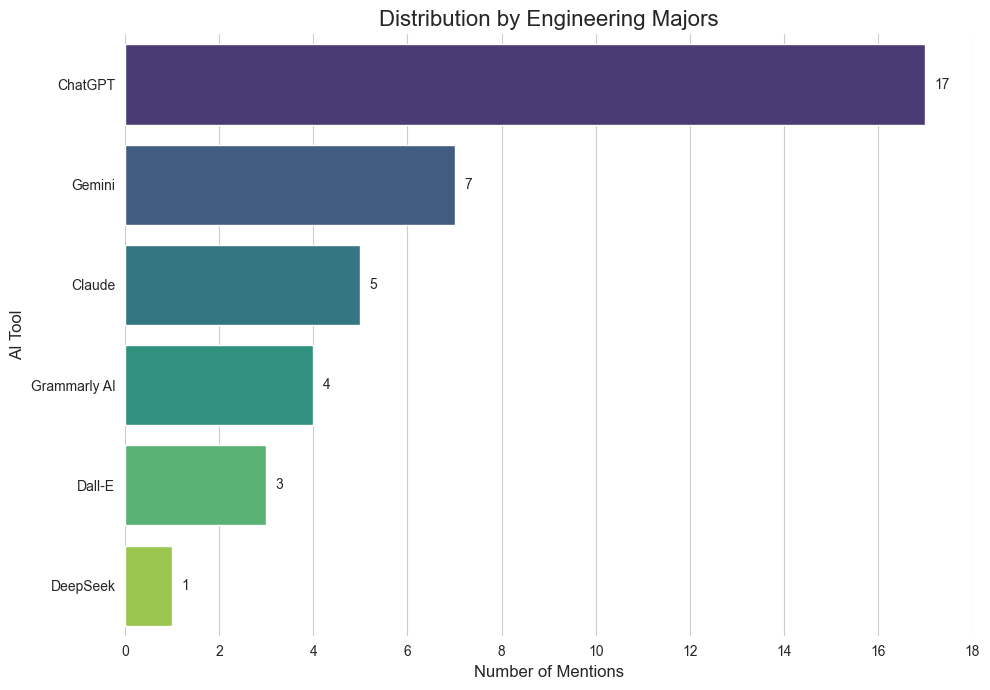
\includegraphics[width=\textwidth]{fig4-1.png} % Replace with your first subfigure file name
    %\caption{Description of subfigure (a)}
    \label{fig:subfig1a}
  \end{subfigure}
  \hfill % Add some horizontal space between the subfigures
  \begin{subfigure}[b]{0.45\textwidth}
    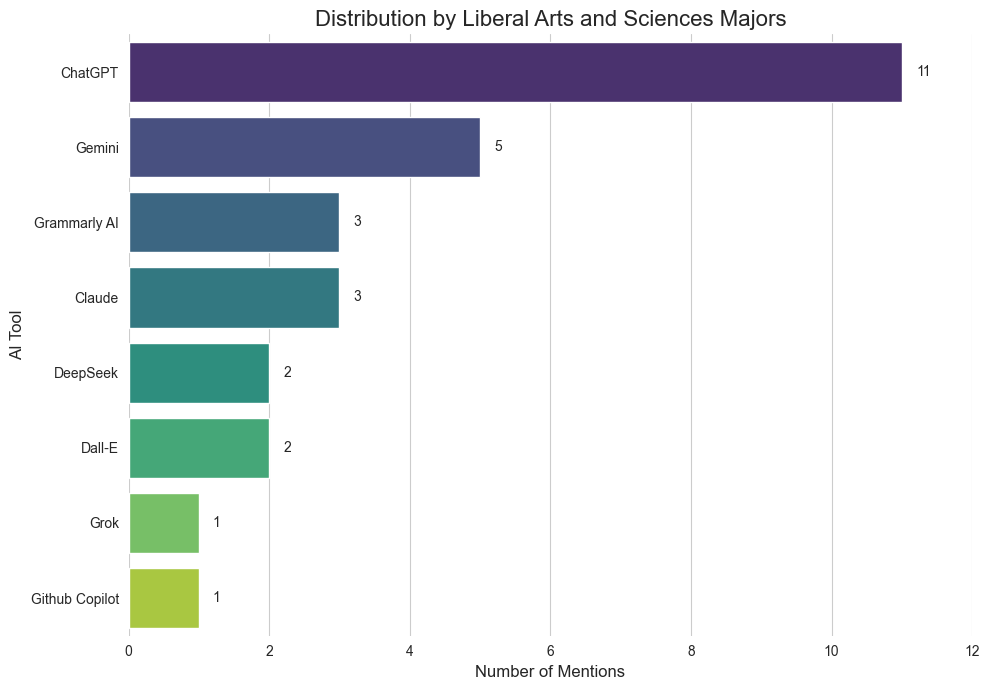
\includegraphics[width=\textwidth]{fig4-2.png} % Replace with your second subfigure file name
    %\caption{Description of subfigure (b)}
    \label{fig:subfig1b}
  \end{subfigure}
  \hfill % Add some horizontal space between the subfigures
  \begin{subfigure}[b]{0.45\textwidth}
    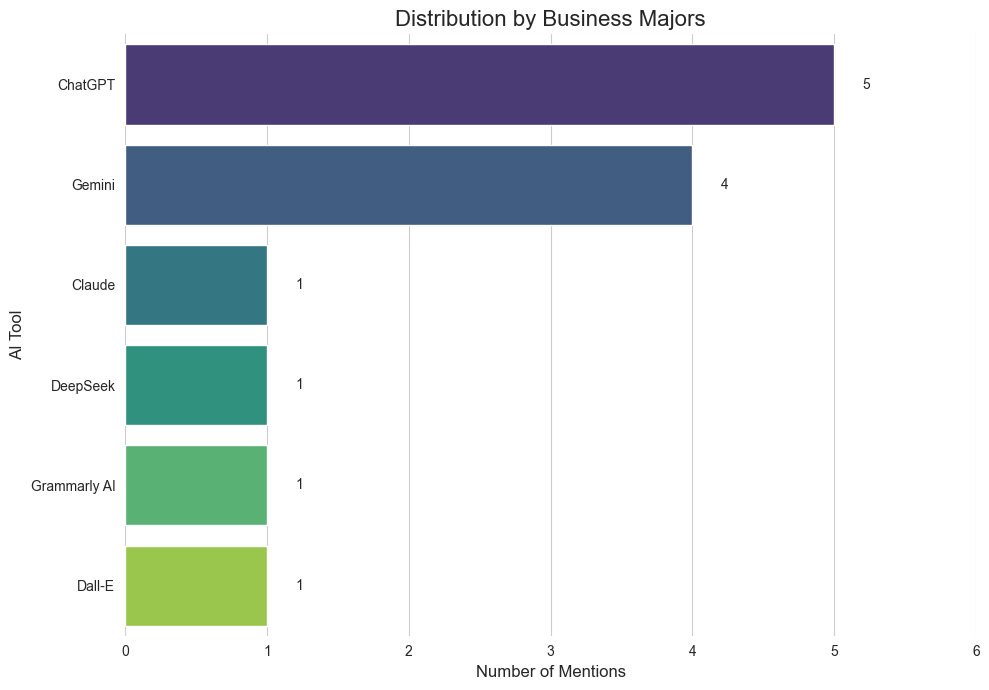
\includegraphics[width=\textwidth]{fig4-3.png} % Replace with your second subfigure file name
    %\caption{Description of subfigure (b)}
    \label{fig:subfig1b}
  \end{subfigure}
  \hfill % Add some horizontal space between the subfigures
  \begin{subfigure}[b]{0.45\textwidth}
    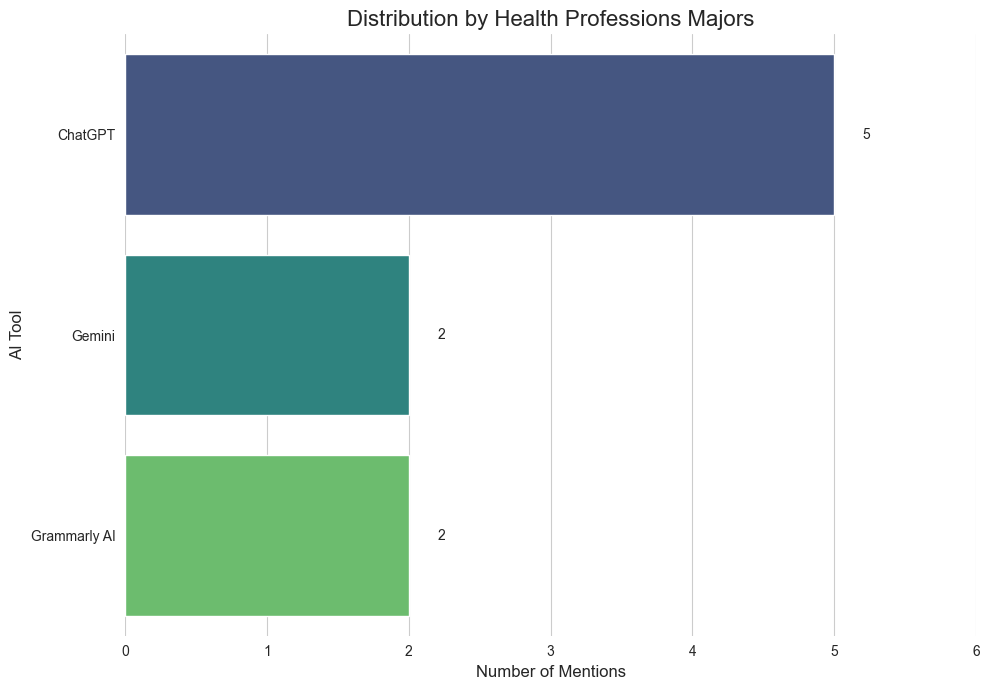
\includegraphics[width=\textwidth]{fig4-4.png} % Replace with your second subfigure file name
    %\caption{Description of subfigure (b)}
    \label{fig:subfig1b}
  \end{subfigure}
  \caption{Comparison of AI tool usage by major.}
  \label{fig:subfigures1}
\end{figure}


Participants reported using AI for a wide variety of academic tasks. Writing and editing was the most frequently cited use, selected by 87\% of respondents. Other common applications included research and information gathering (74\%), studying and note-taking (62\%), and math or problem solving (59\%). Additional uses included career development (46\%), coding (41\%), productivity and organization (26\%), data analysis (21\%), and content creation (18\%) (Figure 5).


\begin{figure}[htbp]
  \centering
  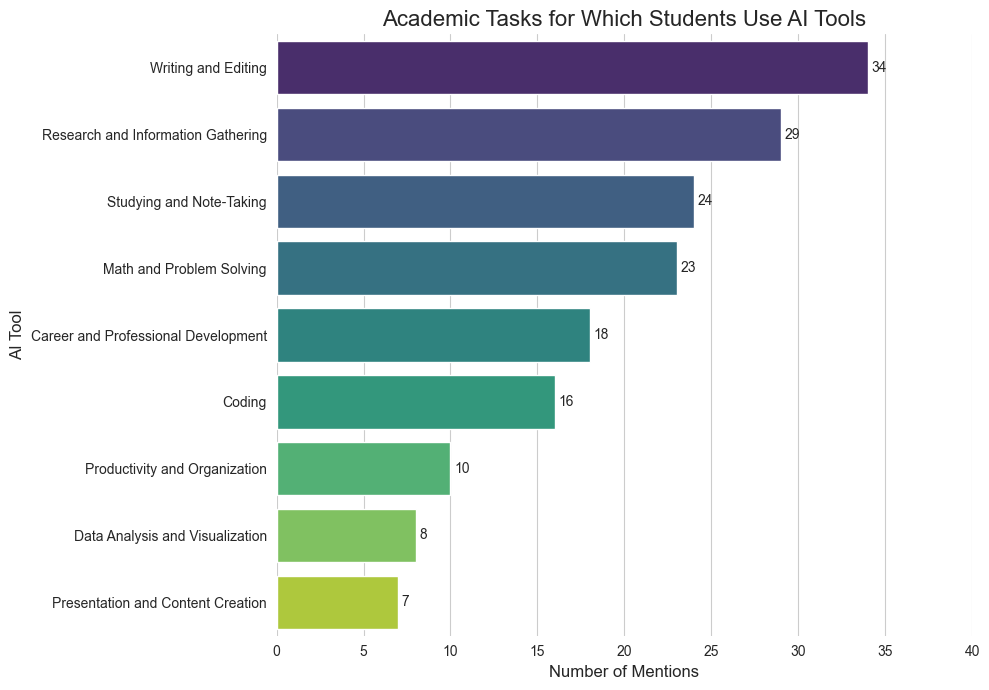
\includegraphics[width=0.69\textwidth]{fig5.png} % Replace with your figure file name
  \caption{Frequency chart of AI usage for various academic tasks.}
  \label{fig:example1}
\end{figure}

Figure 6 provides further detail on how usage patterns differed by academic discipline. Among engineering majors, the top responses were writing and editing (14), math and problem solving (14), coding (12), and research and information gathering (11). Liberal arts and sciences majors most commonly reported writing and editing (10), studying and note-taking (10), and research and information gathering (8). For business and health professions majors, writing and editing (5) and research and information gathering (5) were the most frequent responses.


% Example of two subfigures side-by-side
\begin{figure}[H]
  \centering
  \begin{subfigure}[b]{0.49\textwidth}
    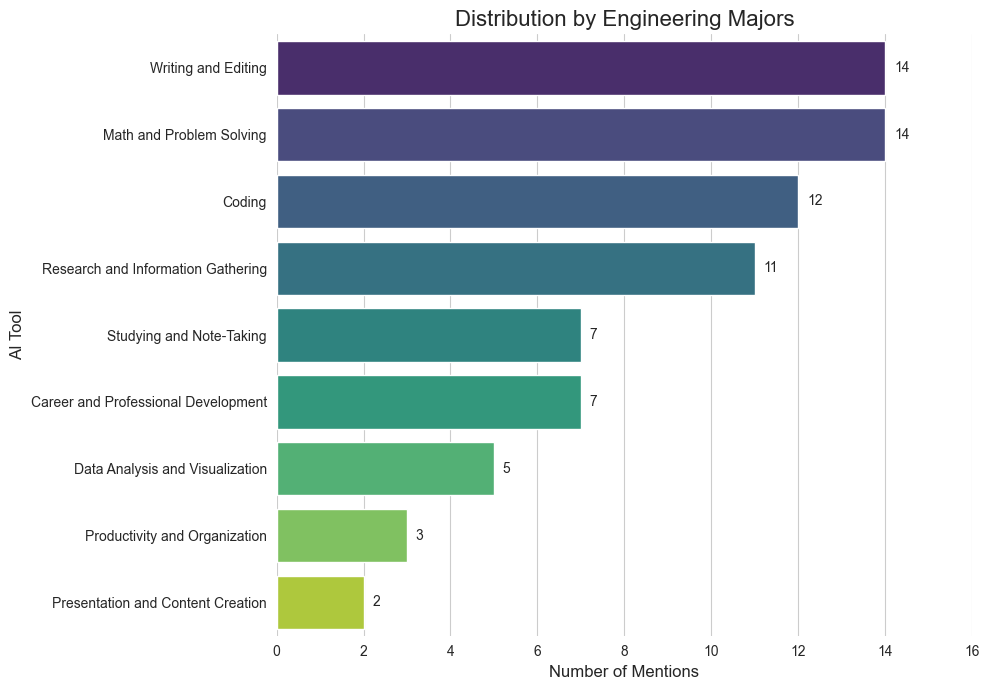
\includegraphics[width=\textwidth]{fig6-1.png} % Replace with your first subfigure file name
    %\caption{Description of subfigure (a)}
    \label{fig:subfig1a}
  \end{subfigure}
  \begin{subfigure}[b]{0.49\textwidth}
    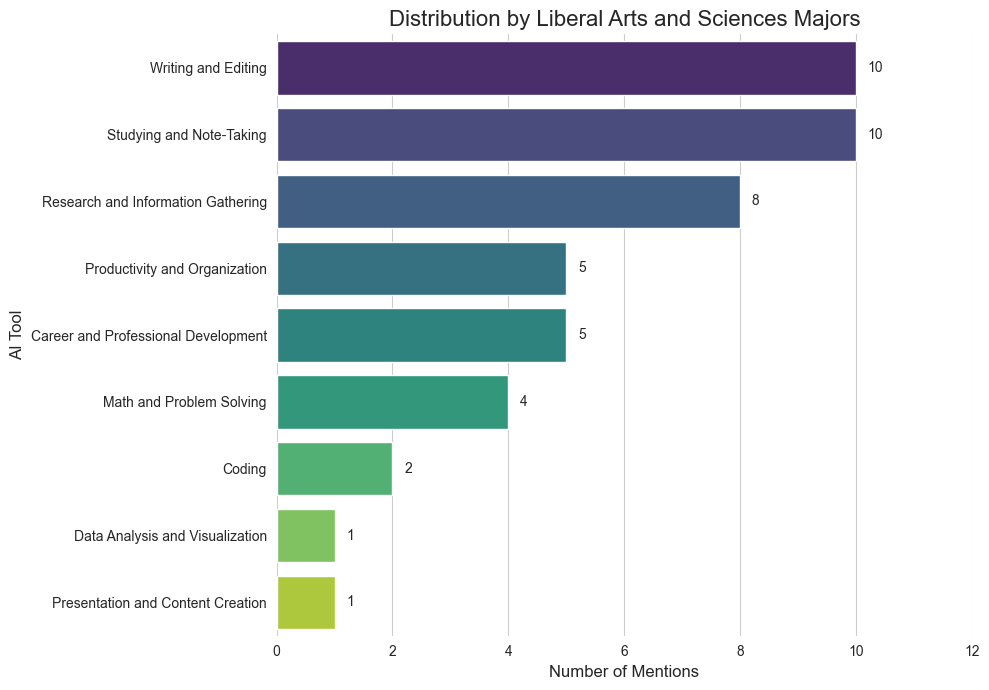
\includegraphics[width=\textwidth]{fig6-2.png} % Replace with your second subfigure file name
    %\caption{Description of subfigure (b)}
    \label{fig:subfig1b}
  \end{subfigure}
  \begin{subfigure}[b]{0.49\textwidth}
    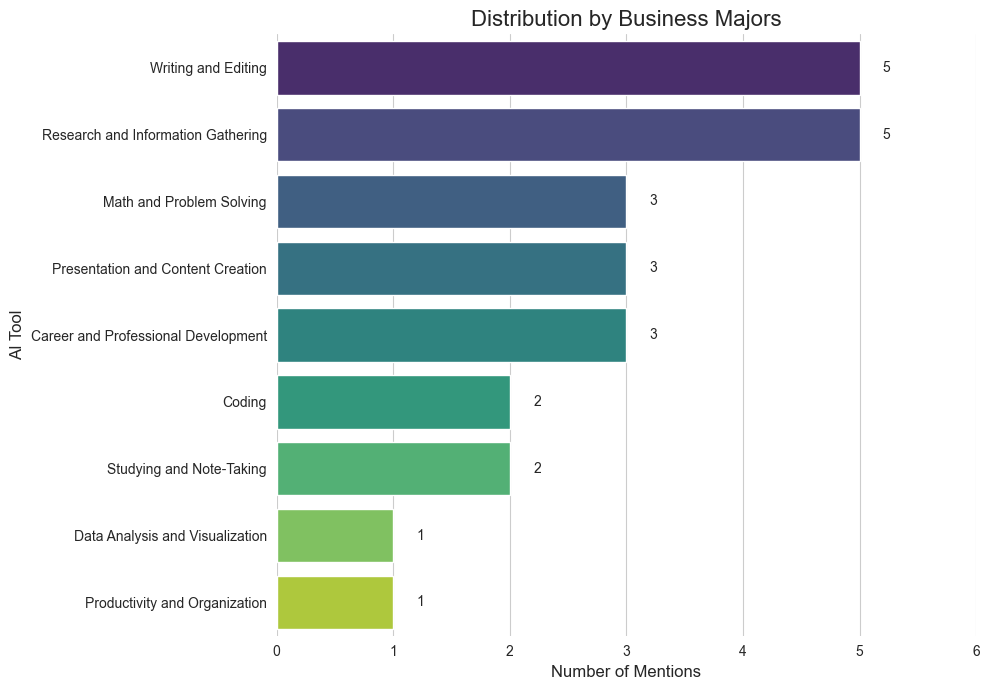
\includegraphics[width=\textwidth]{fig6-3.png} % Replace with your second subfigure file name
    %\caption{Description of subfigure (b)}
    \label{fig:subfig1b}
  \end{subfigure}
  \begin{subfigure}[b]{0.49\textwidth}
    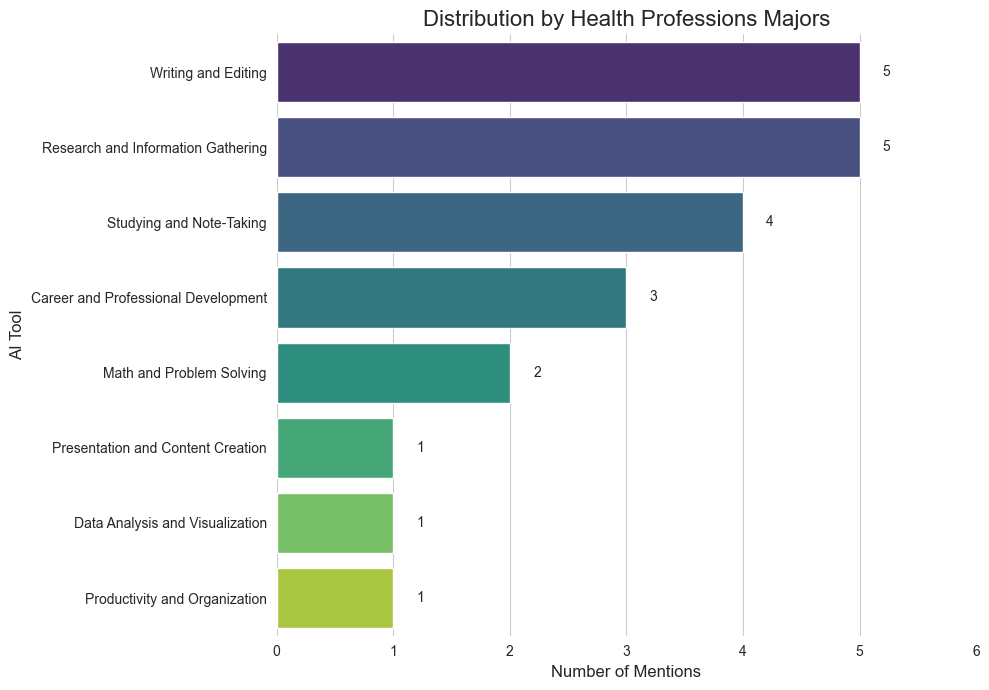
\includegraphics[width=\textwidth]{fig6-4.png} % Replace with your second subfigure file name
    %\caption{Description of subfigure (b)}
    \label{fig:subfig1b}
  \end{subfigure}
  \caption{Comparison of AI usage for various academic tasks by major.}
  \label{fig:subfigures1}
\end{figure}


The survey also included three attitudinal statements rated on a five-point Likert scale. In response to “AI improves my learning experience as a student,” 19 participants strongly agreed, 13 somewhat agreed, 4 neither agreed nor disagreed, 2 somewhat disagreed, and 1 strongly disagreed (Figure 7).

\begin{figure}[htbp]
  \centering
  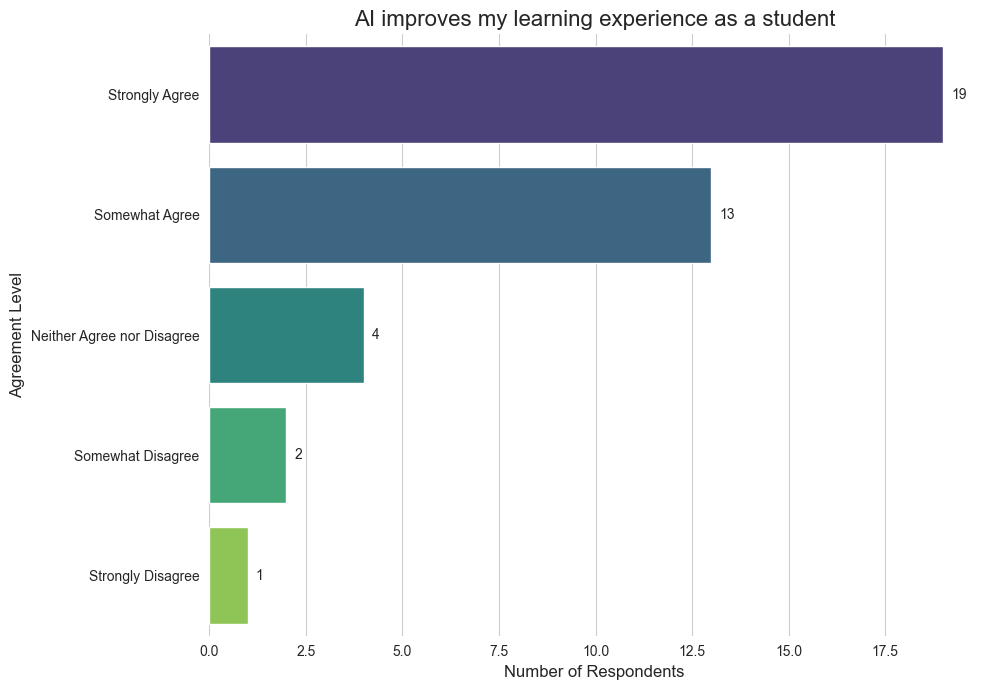
\includegraphics[width=0.7\textwidth]{fig7.png} % Replace with your figure file name
  \caption{\centering Frequency chart of responses to the statement “AI improves my learning experience as a student.”}
  \label{fig:example1}
\end{figure}

For “AI tools are accessible to me,” responses were predominantly positive: 23 strongly agreed, 15 somewhat agreed, and 2 neither agreed nor disagreed (Figure 8).

\begin{figure}[htbp]
  \centering
  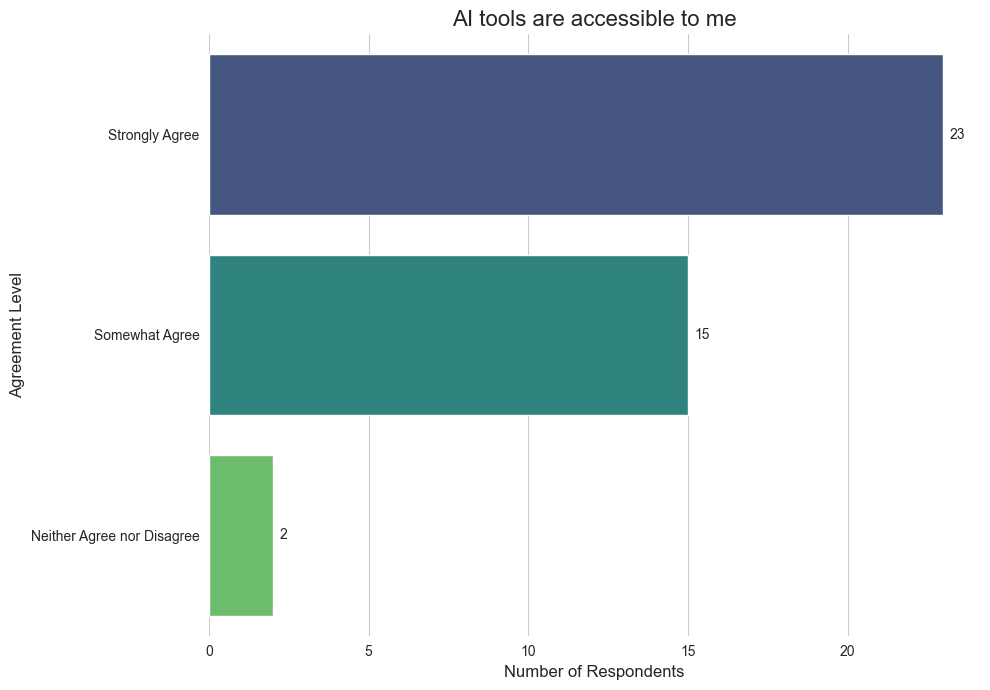
\includegraphics[width=0.7\textwidth]{fig8.png} % Replace with your figure file name
  \caption{\centering Frequency chart of responses to the statement “AI tools are accessible to me.”}
  \label{fig:example1}
\end{figure}

Responses to the final statement, “AI tools are more beneficial in my field of study compared to others,” were mixed: 17 participants selected “Neither Agree nor Disagree,” 10 “Somewhat Agree,” 9 “Strongly Agree,” and 4 “Somewhat Disagree” (Figure 9). When broken down by major, engineering students most commonly selected “Somewhat Agree” (8 responses), whereas students from other fields most frequently chose “Neither Agree nor Disagree” (Figure 10).

\begin{figure}[htbp]
  \centering
  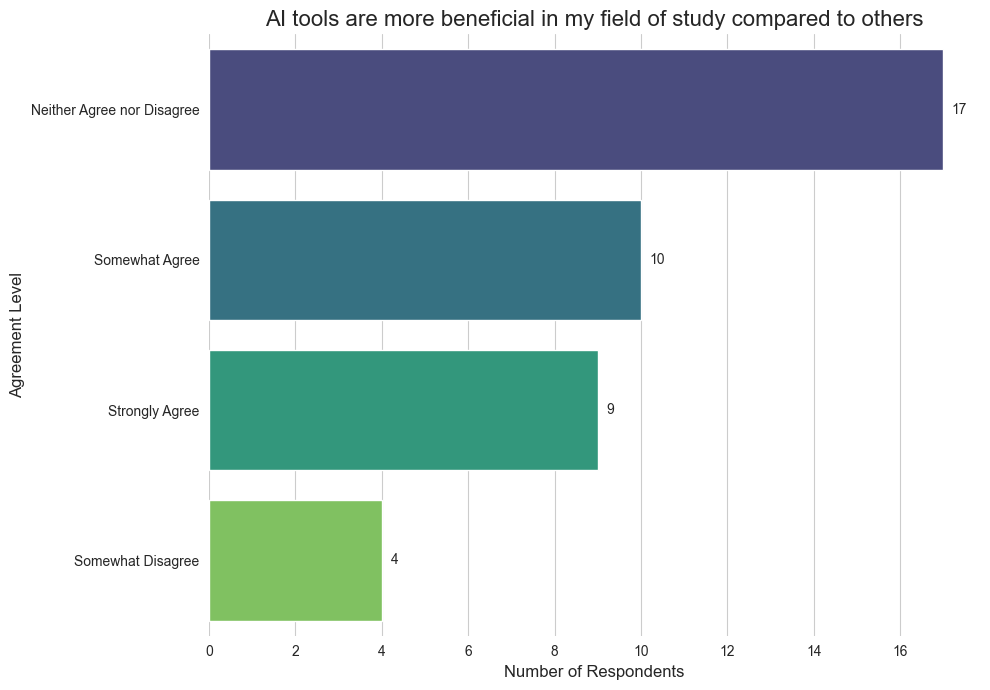
\includegraphics[width=0.5\textwidth]{fig9.png} % Replace with your figure file name
  \caption{\centering Frequency chart of responses to the statement “AI tools are more beneficial in my field of study compared to others.”}
  \label{fig:example1}
\end{figure}

% Example of two subfigures side-by-side
\begin{figure}[htbp]
  \centering
  \begin{subfigure}[b]{0.45\textwidth}
    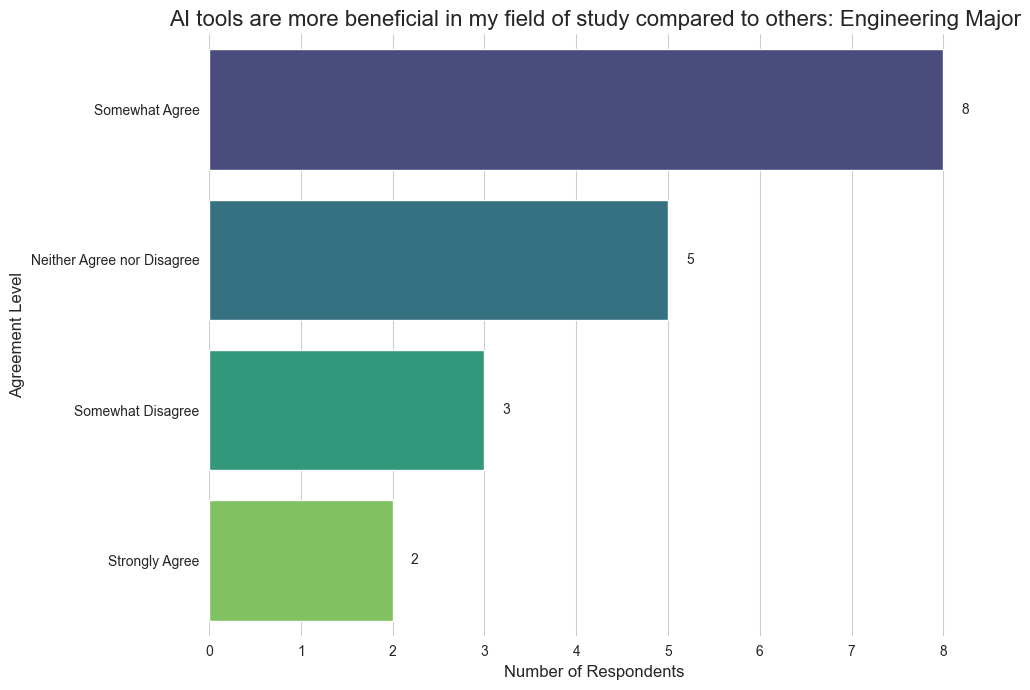
\includegraphics[width=\textwidth]{fig10-1.png} % Replace with your first subfigure file name
    %\caption{Description of subfigure (a)}
    \label{fig:subfig1a}
  \end{subfigure}
  \hfill % Add some horizontal space between the subfigures
  \begin{subfigure}[b]{0.45\textwidth}
    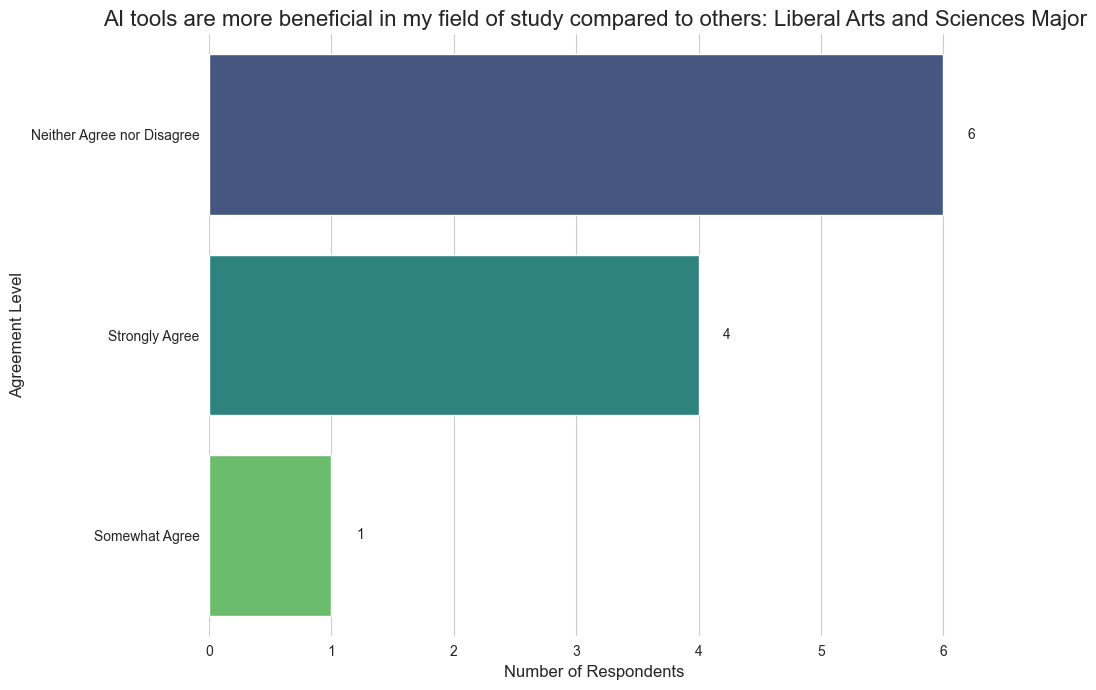
\includegraphics[width=\textwidth]{fig10-2.png} % Replace with your second subfigure file name
    %\caption{Description of subfigure (b)}
    \label{fig:subfig1b}
  \end{subfigure}
  \hfill % Add some horizontal space between the subfigures
  \begin{subfigure}[b]{0.45\textwidth}
    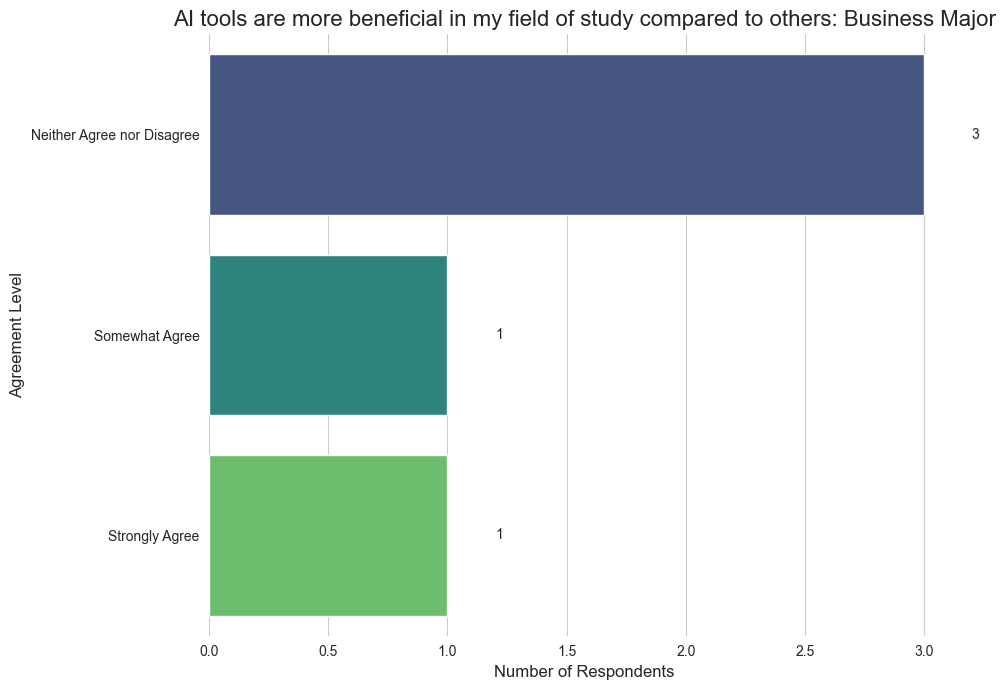
\includegraphics[width=\textwidth]{fig10-3.png} % Replace with your second subfigure file name
    %\caption{Description of subfigure (b)}
    \label{fig:subfig1b}
  \end{subfigure}
  \hfill % Add some horizontal space between the subfigures
  \begin{subfigure}[b]{0.45\textwidth}
    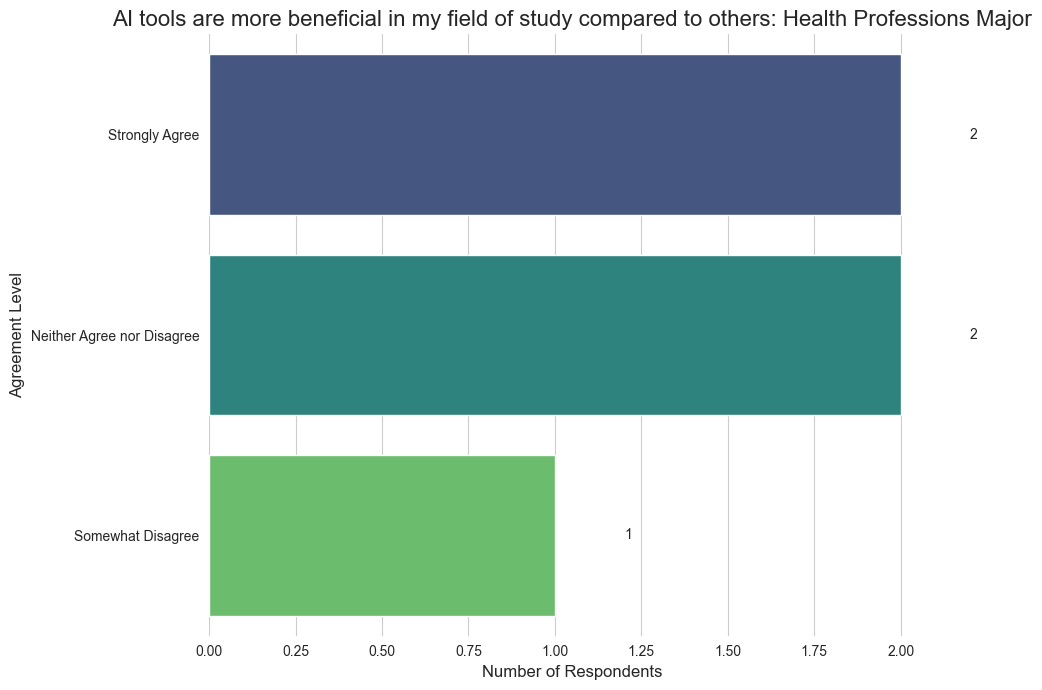
\includegraphics[width=\textwidth]{fig10-4.png} % Replace with your second subfigure file name
    %\caption{Description of subfigure (b)}
    \label{fig:subfig1b}
  \end{subfigure}
  \caption{\centering Comparison of responses to the statement “AI tools are more beneficial in my field of study compared to others” by major.}
  \label{fig:subfigures1}
\end{figure}

% --- Discussion ---
\section{Discussion and Conclusion}
\label{sec:discussion_and_conclusion}
Overall, the data suggest that AI tools are widely used across academic disciplines, with particularly high engagement among engineering and liberal arts students. ChatGPT emerged as the dominant tool, while other tools such as Gemini, Grammarly AI, and Claude showed varied adoption based on field of study. Writing and editing tasks were the most common use case, but a diverse range of applications—from coding to studying—highlights the adaptability of AI across academic fields.
These findings align with existing literature on the versatility of AI in education \cite{pedro, md} but offer a more nuanced look at how engagement differs by discipline. Engineering students, for example, showed relatively high use of technical tools like Claude and DeepSeek, while liberal arts students favored Grammarly AI. This supports the idea that students tailor their AI use to the specific needs of their academic discipline \cite{lin}. Inferences regarding the usage patterns of other groups (Business, Health Professions, Law Professions, and Agriculture) cannot be drawn due to statically insignificant sample sizes.
Students’ attitudes toward AI were generally positive, with most agreeing that AI enhances their learning experience and is easily accessible, echoing the findings of C. K. Y. Chan et al. \cite{chan}, who observed that students across various disciplines view AI as a helpful and accessible tool for academic tasks. However, responses were more divided when participants were asked whether AI tools are particularly beneficial within their specific field of study. Notably, engineering majors were more likely to view AI as especially beneficial in their field, with 8 respondents expressing agreement. This suggests that engineering students may perceive a stronger connection between AI tools and their academic work compared to their peers in other disciplines.
Despite the valuable insights provided by this study, several limitations must be acknowledged. The sample size was relatively small (n = 43), and engineering majors were overrepresented, which limits the generalizability of the findings. Additionally, the broad categorization of academic disciplines may have obscured important distinctions between subfields. For example, while 12 engineering majors reported using AI for coding, it is unclear how many of those were specifically Computer Science majors, a group that may have distinct patterns of AI use compared to other engineering disciplines. These finer distinctions could provide a more nuanced understanding of AI adoption and usage patterns within specific subfields.
Future research should aim for a larger and more balanced sample, possibly incorporating interviews to better understand how students’ use of AI evolves over time. Moreover, deeper investigation into the pedagogical, and cognitive implications of AI in discipline-specific contexts would help inform institutional policies and instructional design.
In conclusion, this study offers early insight into the ways AI is reshaping student engagement across academic fields. Understanding these patterns is essential not only for aligning educational strategies with student needs but also for preparing institutions to adapt to the evolving role of AI in higher education.


\pagebreak

% Example using a simple \thebibliography environment:
\begin{thebibliography}{9}
  \bibitem{am} A. M. Vieriu and G. Petrea, ‘The Impact of Artificial Intelligence (AI) on Students’ Academic Development’, \textit{Education Sciences}, vol. 15, no. 3, 2025.
  \bibitem{pedro} F. Pedro, M. Subosa, A. Rivas, and P. Valverde, "Artificial intelligence in education: challenges and opportunities for sustainable development," UNESCO, Paris, France, 2019. [Online]. Available: https://unesdoc.unesco.org/ark:/48223/pf0000366994
  \bibitem{lin} X. Lin, R. Chan, S. Sharma, and K. Bista, ChatGPT and Global Higher Education: Using Artificial Intelligence in Teaching and Learning. \textit{Star Scholars Press}, 2024. 
  \bibitem{md} M. D. Adewale, A. Azeta, A. Abayomi-Alli, and A. Sambo-Magaji, ‘Impact of artificial intelligence adoption on students’ academic performance in open and distance learning: A systematic literature review’, \textit{Heliyon}, vol. 10, no. 22, p. e40025, 2024.
  \bibitem{chan} C. K. Y. Chan and W. Hu, "Students' voices on generative AI: perceptions, benefits, and challenges in higher education," Int. J. Educ. Technol. High. Educ., vol. 20, no. 1, p. 43, 2023.
\end{thebibliography}

% --- Appendices (Optional) ---
\appendix
\section{Appendix: Survey}
\begin{figure}[H]
  \centering
  \begin{subfigure}[b]{0.49\textwidth}
    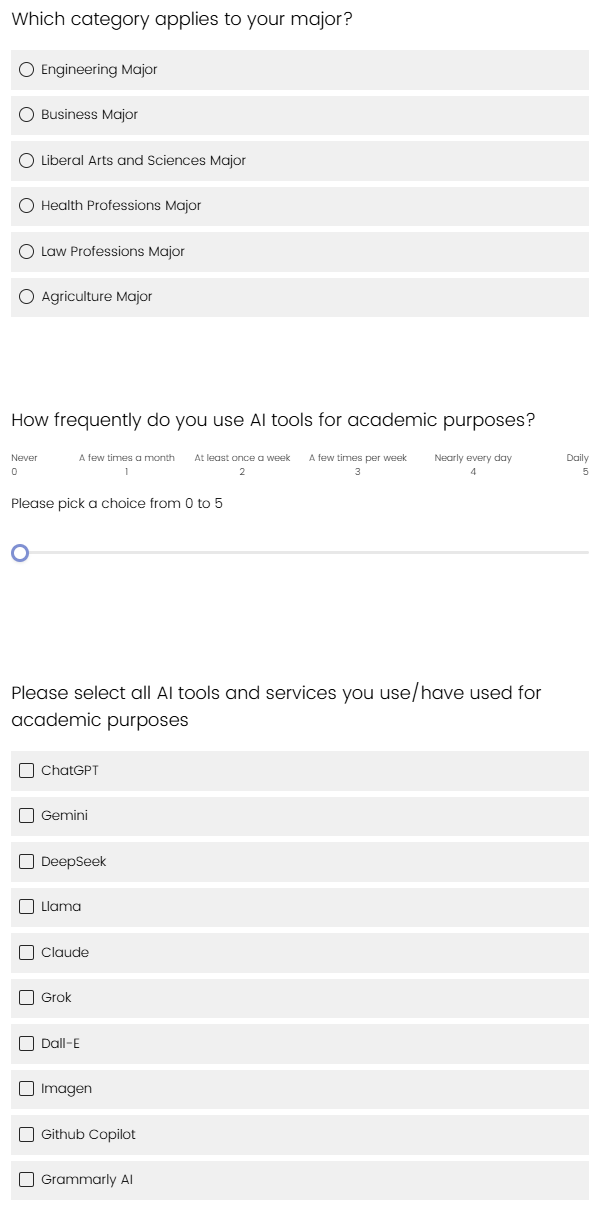
\includegraphics[width=\textwidth]{s1.png} % Replace with your first subfigure file name
    %\caption{Description of subfigure (a)}
    \label{fig:subfig1a}
  \end{subfigure}
  \begin{subfigure}[b]{0.49\textwidth}
    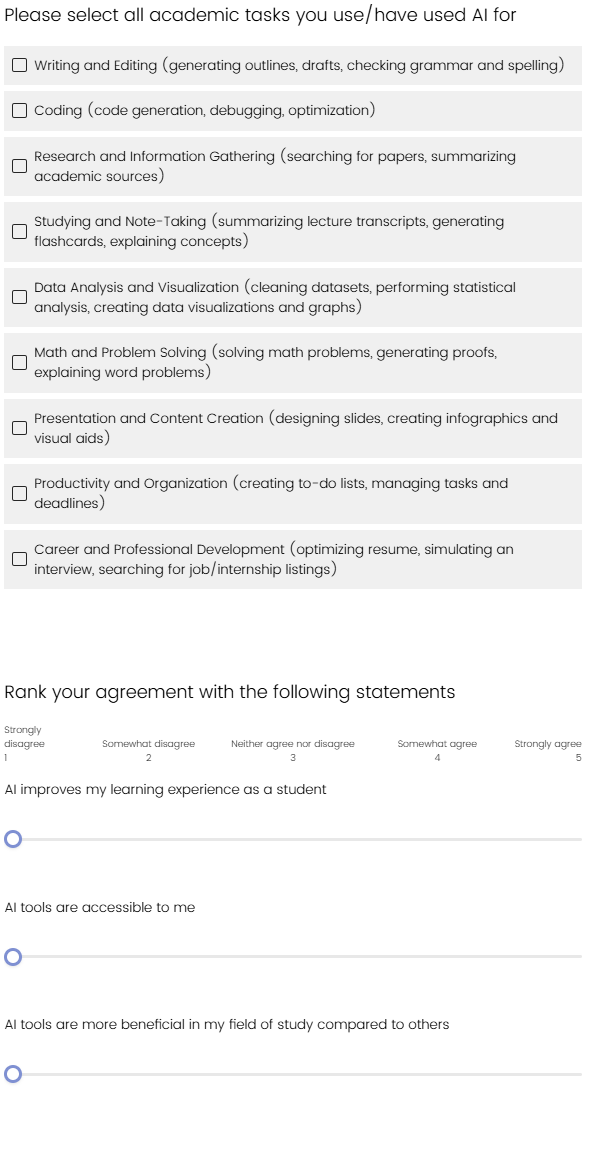
\includegraphics[width=\textwidth]{s2.png} % Replace with your second subfigure file name
    %\caption{Description of subfigure (b)}
    \label{fig:subfig1b}
  \end{subfigure}
  \caption{Overall caption for the two subfigures.}
  \label{fig:subfigures1}
\end{figure}
\section{Appendix: Data Analysis Repository}
The full code, dataset, and analysis for this study are available on GitHub:
\url{https://github.com/mauricio-b-mossi/ResearchReportDataAnalysisENC3246/tree/main}
% --- End Document ---
\end{document}